%% LaTeX-Beamer template for KIT design
%% by Erik Burger, Christian Hammer
%% title picture by Klaus Krogmann
%%
%% version 2.0
%%
%% mostly compatible to KIT corporate design v2.0
%% http://intranet.kit.edu/gestaltungsrichtlinien.php
%%
%% Problems, bugs and comments to
%% burger@kit.edu

\documentclass[18pt]{beamer}
\usetheme{kit}

\titleimage{titleImage}
\titlelogo{logos}

% the presentation starts here

\title[MDP Pfadplanung]{Markov-Entscheidungsprozesse für die Roboterpfadplanung}
\subtitle{Entscheidungsprobleme unter Unsicherheit} %TODO nötig?
\author{Matthias Holoch}

\institute{Proseminar Anthropomatik: Von der Theorie zur Anwendung}

\begin{document}

\selectlanguage{ngerman}

%title page
\begin{frame}
	\titlepage
\end{frame}

%table of contents %TODO remove it, maybe
\frame{
	\frametitle{Gliederung}
	\tableofcontents
}


\section{Einleitung}
\subsection{Wozu das Ganze?}
\begin{frame}
	\frametitle{Wozu das Ganze?}
	\begin{itemize}
		\item Lösen von Entscheidungsproblemen 
		\begin{itemize}
			\item Einbezug von Unsicherheiten
		\end{itemize}
		\visible<2->{
		\item Medizinische Diagnose
		\begin{itemize}
			\item genauer Patientenzustand unbekannt
			\item Menge an Therapiemöglichkeiten
			\item Beobachtungen als Hinweis auf den Patientenzustand
			\item Abwägen von Kosten
		\end{itemize}
		}
		\visible<3->{
		\item Roboterpfadplanung
		}
	\end{itemize}
\end{frame}


\section{Planung unter Unsicherheit}
\subsection{Planung klassisch}
\begin{frame}
	\frametitle{Klassische Pfadplanung}	
	\visible<2->{
		\only<1,2>{
			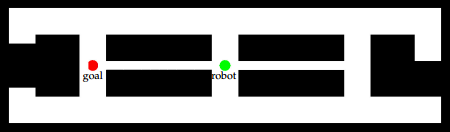
\includegraphics[scale=0.8]{images/autnmRobot_basicSituation.png}
		}
		\only<3->{
			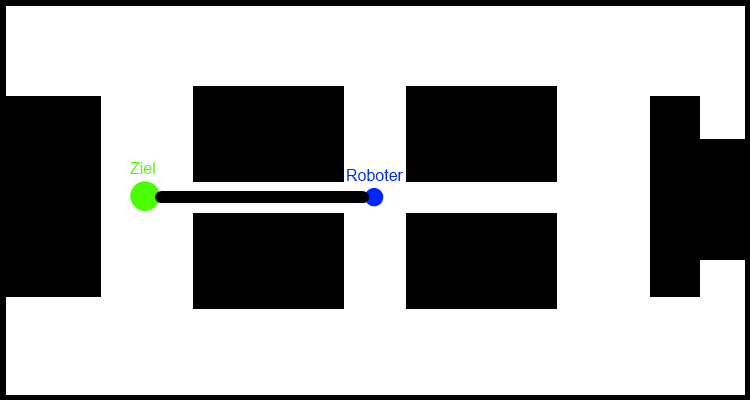
\includegraphics[scale=0.8]{images/autnmRobot_directPath.png}
		}
	}
	\only<-4>{
		\\Annahmen
		\begin{enumerate}
			\item Genauer Zustand erkennbar
			\item Aktionsausführung fehlerfrei
		\end{enumerate}
		\visible<4->{
			Probleme
			\begin{itemize}
				\item Fehler im Bewegungsmodell
				\item Schlupf zwischen Antriebsrädern und Untergrund
				\item verrauschte Sensordaten
			\end{itemize}
		}
	}
	\only<5->{
		\\ Aktionsausführung nicht fehlerfrei, genauer Zustand nicht erkennbar.
		\begin{itemize}
			\item Verlassen des geplanten Pfads
			\item häufige Korrektur
			\item erhöhtes Messintervall bei engen Korridoren
		\end{itemize}
		\visible<6>{
			\textbf{Einzelne Aktionsfolge reicht nicht aus.}
		}
	}
\end{frame}

\subsection{Pfadplanung mit MDPs}
\begin{frame}
	\frametitle{Pfadplanung mit MDPs}
	\visible<3->{
		\only<1,2,3>{
			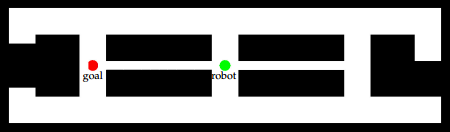
\includegraphics[scale=0.8]{images/autnmRobot_basicSituation.png}
		}
		\only<4>{
			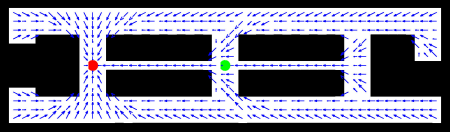
\includegraphics[scale=0.8]{images/autnmRobot_detActionMDP.png}
		}
		\only<5>{
			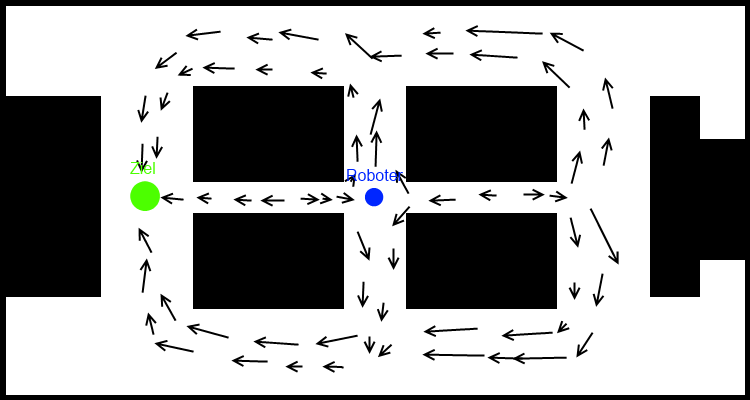
\includegraphics[scale=0.8]{images/autnmRobot_ndetActionMDP.png}
		}
	}
	\\Annahmen
	\begin{enumerate}
		\item Genauer Zustand erkennbar
	\end{enumerate}
	\visible<2->{
		Vorberechnete Aktionsfolgen
		\begin{itemize}
			\item antizipieren Fehlverhalten
			\item sind \glqq optimal\grqq
		\end{itemize}
	}
\end{frame}


\section{MDP}
\subsection{Formal}
\begin{frame}
	\frametitle{MDP}
	Ein MDP ist ein 4-Tupel
	\begin{equation}
		(S, A, T, r)
	\end{equation}
	mit
	\begin{itemize}
		\visible<1->{
			\item diskreter, endlicher Zustandsmenge $S$
		}
		\visible<2->{
			\item diskreter, endlicher Aktionsmenge $A$
		}		
		\visible<3->{
			\item Zustandsübergangsmodell des Systems $T$
				\begin{equation}
					T(s, a, s') = \mathbf{p}(s'|s, a)
				\end{equation}
		}
		\visible<4->{
			\item Funktion
				\begin{equation}
					r: S \times A \rightarrow \mathbb{R}\ .
				\end{equation}
		}
	\end{itemize}
\end{frame}

\subsection{Beispiel}
\begin{frame}
	\frametitle{MDP Beispiel}
	\only<1>{
		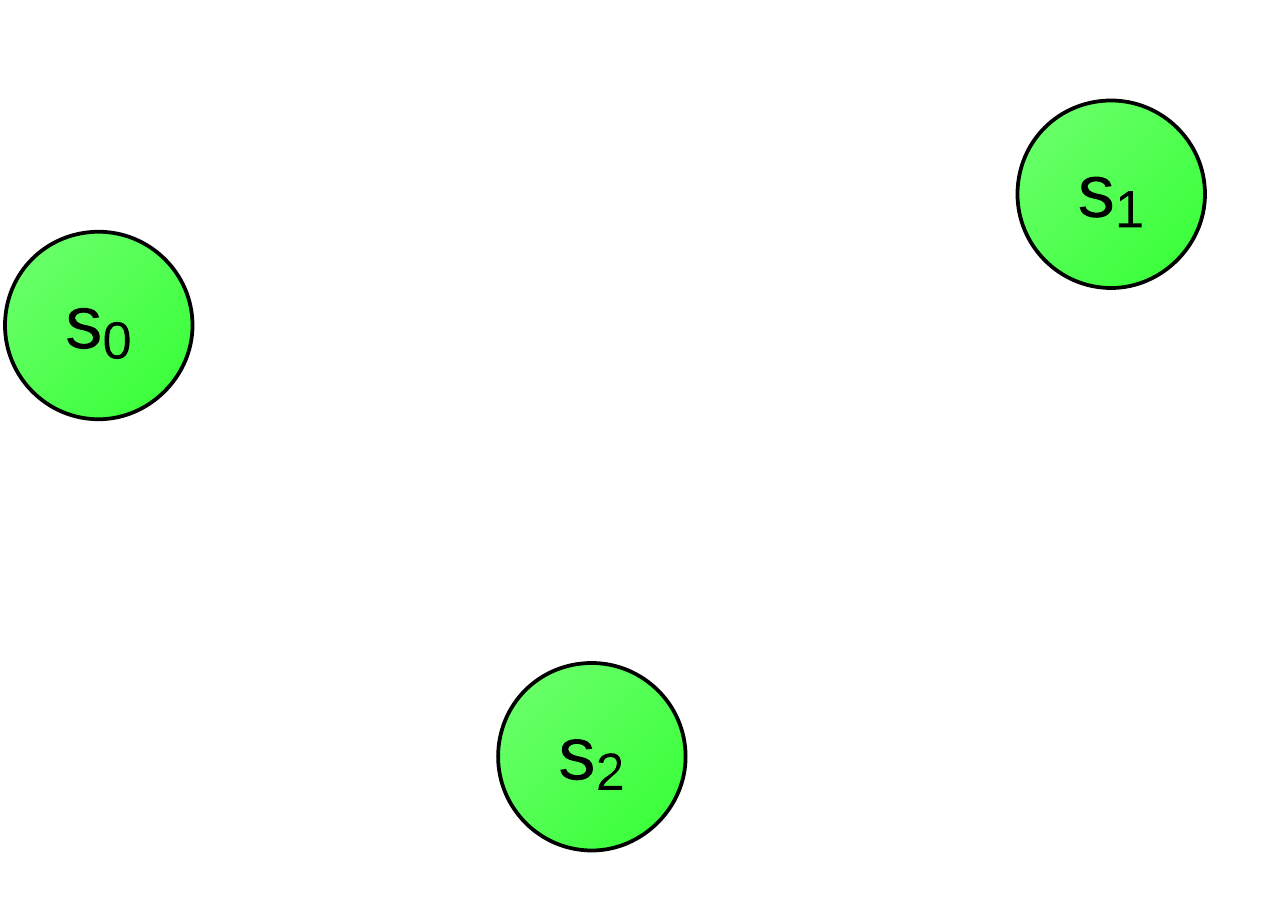
\includegraphics[scale=0.2]{images/MDP_example_part2.png}
	}
	\only<2>{
		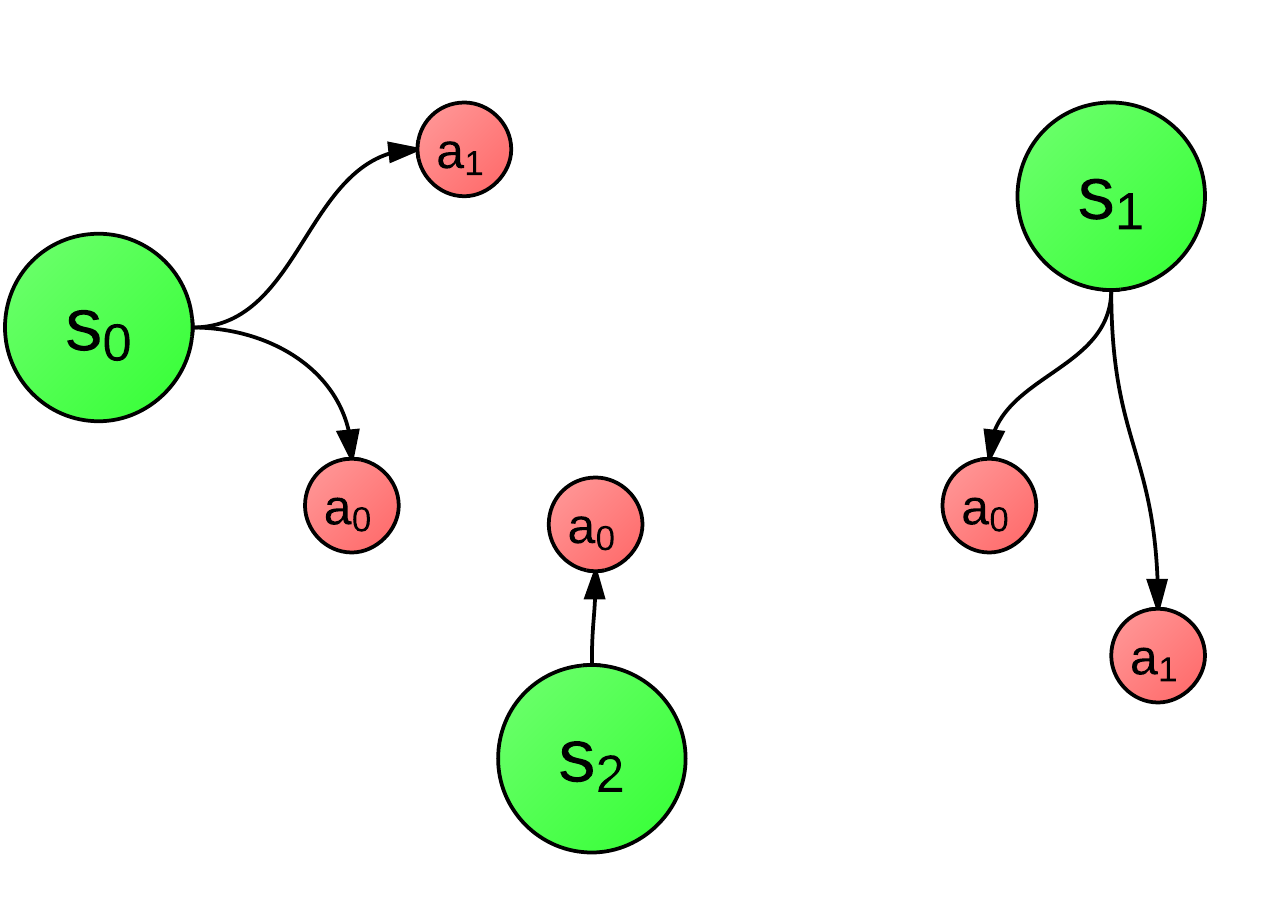
\includegraphics[scale=0.2]{images/MDP_example_part1.png}
	}
	\only<3>{
		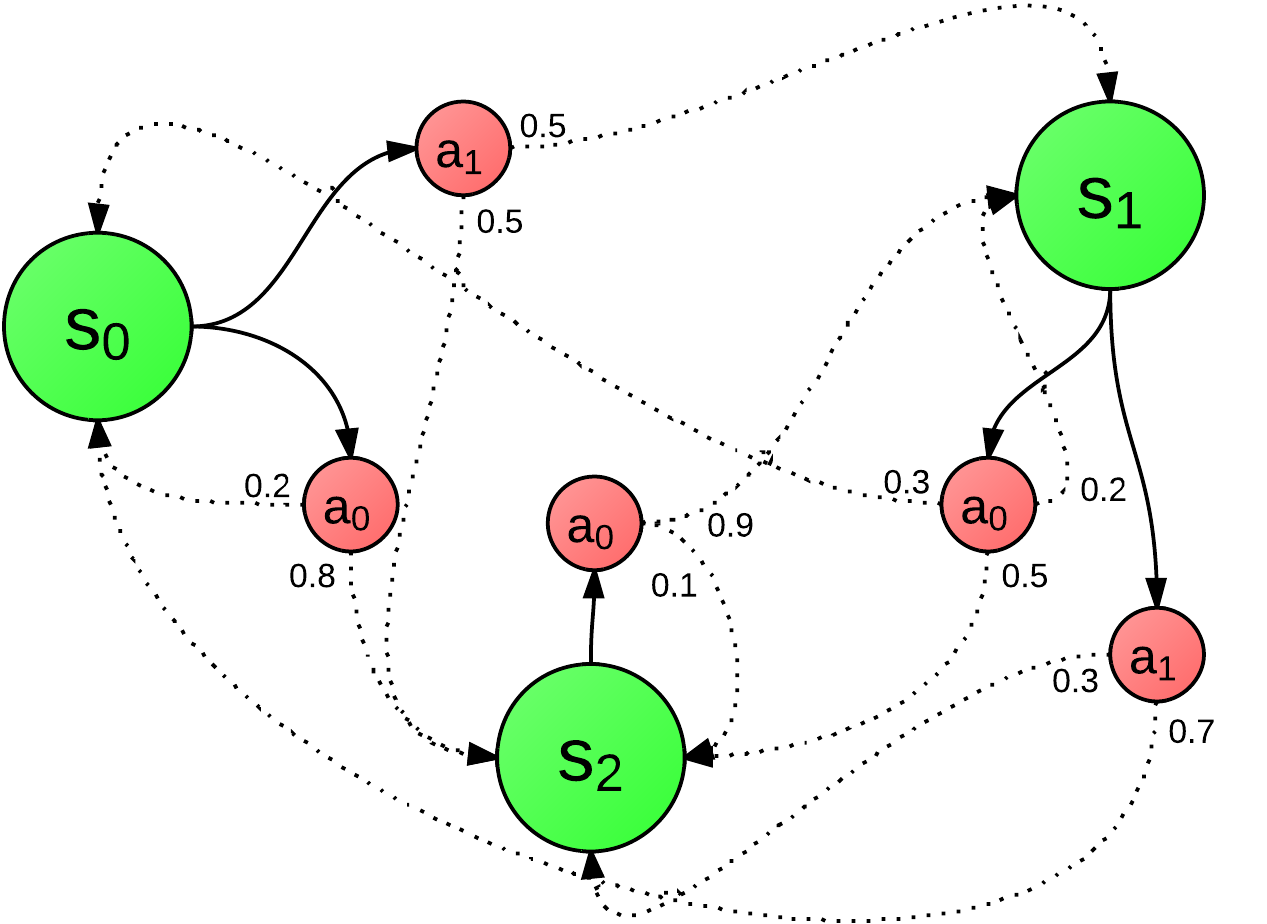
\includegraphics[scale=0.2]{images/MDP_example_part0.png}
	}
	\only<4>{
		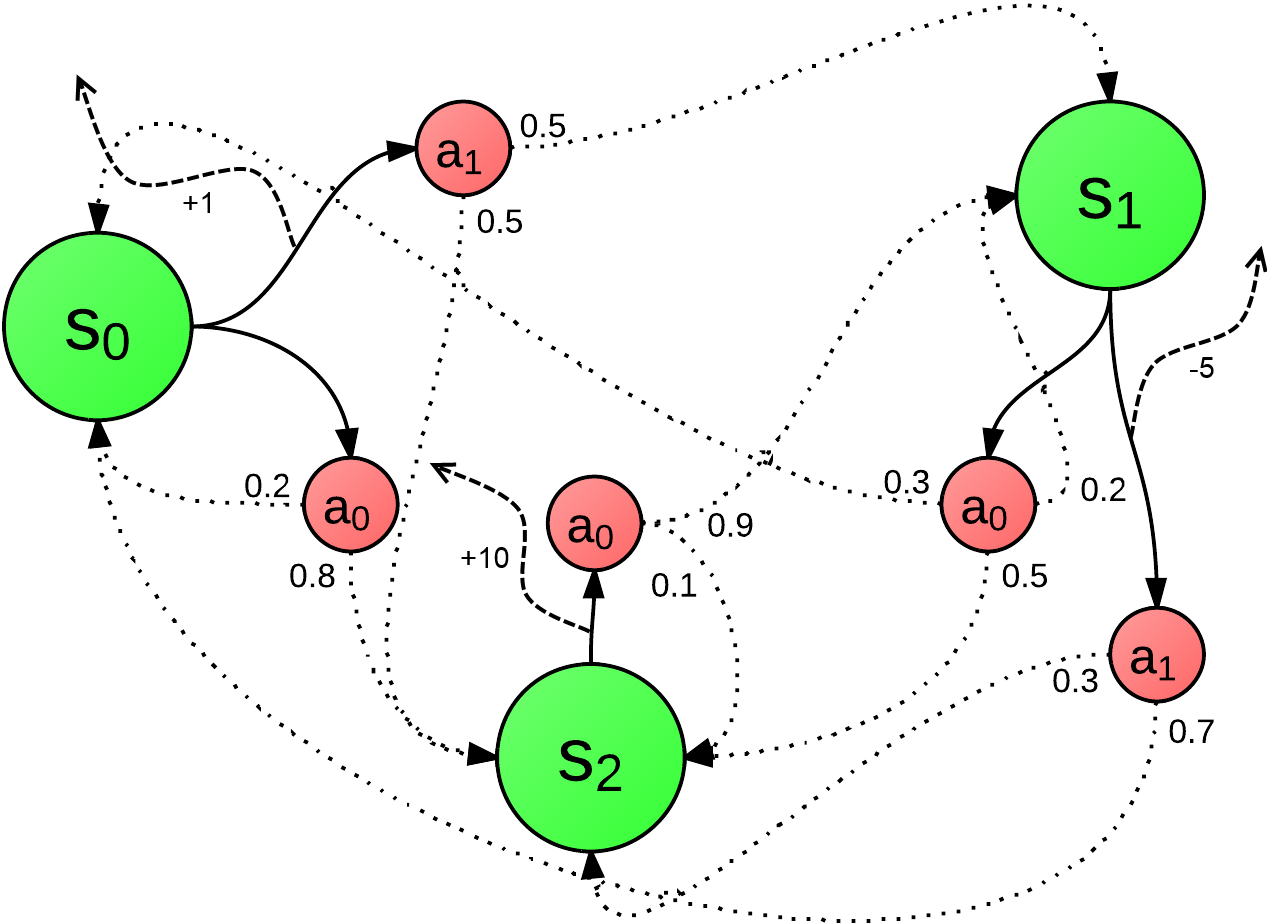
\includegraphics[scale=0.2]{images/MDP_example.png}
	}
	\begin{itemize}
	\visible<1->{
		\item $S = \{s_0, s_1, s_2\}$
	}
	\visible<2->{
		\item $A = \{a_0, a_1\}$
	}
	\visible<3->{
		\item $T(s_0, a_0, s_0) = 0.2;\ T(s_0, a_0, s_1) = 0.8;\ ...$
	}
	\visible<4->{
		\item $r(s_0, a_1) = 1;\ r(s_2, a_0) = 10;\ r(s_1, a_1) = -5$
	}
	\end{itemize}
\end{frame}

\section{Strategien}
\subsection{Optimale Strategien}
\begin{frame}
	\frametitle{Strategien}
	\only<1>{
		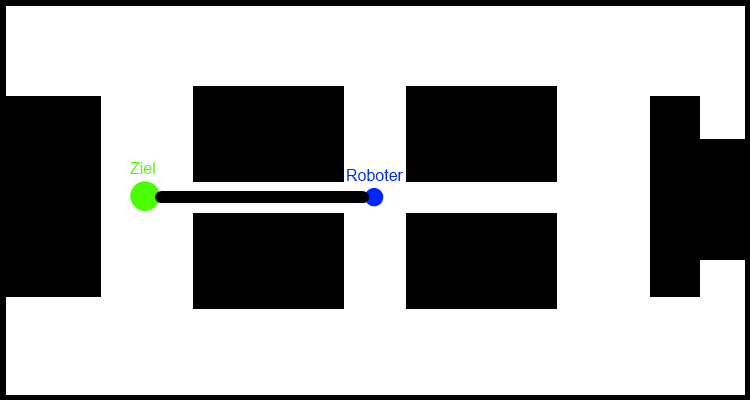
\includegraphics[scale=0.8]{images/autnmRobot_directPath.png}\\
	}
	\only<2->{
		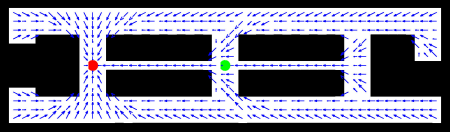
\includegraphics[scale=0.8]{images/autnmRobot_detActionMDP.png}\\
	}
	\visible<3->{
	\vspace{1cm}
		Eine Strategie ist eine Funktion
		\begin{equation}
			\pi: S \rightarrow A\ .
		\end{equation}
	}
\end{frame}
\begin{frame}
	\only<1, 3->{
		\frametitle{Optimale Strategien}
	}
	\only<2>{
		\frametitle{\glqq Optimale\grqq\ Strategien?!}
	}
	\visible<4->{
	\begin{itemize}
		\item Planungshorizont $n$
		\begin{itemize}
			\item Endlicher Planungshorizont
			\item Unendlicher Planungshorizont
		\end{itemize}
		}
		\visible<5->{
		\item Maximierung einer erwarteten Güte aller Aktionsfolgen \\
			  $\left[(s_0, a_0), (s_1, a_1), ..., (s_n, a_n)\right]$
		\begin{itemize}
			\visible<6->{
				\item additive Güte
				\begin{equation}
					\sum\limits_{t=1}^n r(s_t, a_t)
				\end{equation}
			}
			\visible<7->{
				\item reduzierte Güte
				\begin{equation}
					\sum\limits_{t=1}^n \gamma^t r(s_t, a_t),\ \text{mit }\gamma \in [0,1]
				\end{equation}
			}
			\visible<8->{
				\item durchschnittliche Güte pro Zeitschritt
			}
		\end{itemize}
	\end{itemize}
	}
	\begin{center}
		\visible<3->{$\pi^*$}\visible<5->{$ = \underset{\pi}{argmax}\ \mathrm{E}\left[\visible<9->{\sum\limits_{t=1}^{n} \gamma^t r(s_t, a_t) \ \vert\ \pi}\right]$}
	\end{center}
\end{frame}

\subsection{Algorithmus}
\begin{frame}
	\frametitle{Algorithmus - Vorüberlegung}
	\begin{itemize}
		\only<2,3>{
			\item $n=1$:
				\begin{equation}
					\begin{split}
						\pi_1^*(s)= \underset{a}{argmax}\ r(s, a) \\
						V_1(s) = \gamma\ \underset{a}{max}\ r(s, a)
					\end{split}
				\end{equation}
		}
		\visible<3->{
			\item $n=2$:
				\begin{equation}
					\begin{split}
						\pi_2^*(s) = \underset{a}{argmax} \left[ r(s,a) + \sum_{s' \in S} V_1(s')\ T(s, a, s') \right] \\
						V_2(s) = \gamma\ \underset{a}{max} \left[ r(s,a) + \sum_{s' \in S} V_1(s')\ T(s, a, s') \right]
					\end{split}
				\end{equation}
		}
		\only<4->{
			\item $\forall n > 1$:
				\begin{equation}
					\begin{split}
						\pi_n^*(s) = \underset{a}{argmax} \left[ r(s,a) + \sum_{s' \in S} V_{n-1}(s')\ T(s, a, s') \right] \\
						V_n(s) = \gamma\ \underset{a}{max} \left[ r(s,a) + \sum_{s' \in S} V_{n-1}(s')\ T(s, a, s') \right]
					\end{split}
				\end{equation}
		}
	\end{itemize}
\end{frame}
\begin{frame}
	\frametitle{Algorithmus}
	\begin{itemize}
		\visible<2->{
			\item dynamische Programmierung
		}
		\visible<3->{
			\item Initialisierung
				\begin{equation}
					\hat{V}(s) \leftarrow 0
				\end{equation}
		}
		\visible<4->{
			\item pro Iteration
				\begin{equation}
					\hat{V}(s) \leftarrow \gamma\ \underset{a}{max} \left[ r(s,a) + \sum_{s' \in S} \hat{V}(s')\ T(s, a, s') \right]
				\end{equation}
		}
		\visible<5->{
			\item Bis $\hat{V}$ konvergiert
		}
		\visible<6->{
			\item $\hat{V}$ induziert nun
				\begin{equation}
					\pi(s)^* = \underset{a}{argmax} \left[ r(s,a) + \sum_{s' \in S} \hat{V}(s')\ T(s, a, s') \right]
				\end{equation}
		}
	\end{itemize}
\end{frame}


\section{Schluss}
\subsection{Ausblick}
\begin{frame}
	\frametitle{Ausblick}
	Mit dem MDP
	\begin{itemize}
		\item Unsicherheiten in Aktionen modellieren
		\item optimale Strategie berechnen
	\end{itemize}
	\visible<2->{
		\textbf{Aber}
		\begin{itemize}
			\item Annahme: Genauer Zustand erkennbar
			\item Entspricht \emph{nicht} der Realität
		\end{itemize}
	}
	\visible<3->{
		Ausblick: POMDP
		\begin{itemize}
			\item Erlaubt Unsicherheiten in dem Zustand
			\item Wahrscheinlichkeitsverteilung über alle Zustände
		\end{itemize}
	}
\end{frame}

\subsection{Quellen}
\begin{frame}{~}
\begin{center}
	\textbf{{\LARGE Vielen Dank für Ihre Aufmerksamkeit}}
\end{center}
		\bibliographystyle{plain}
		\bibliography{literatur}
\end{frame}

\end{document}
